Autoformer là 1 mô hình học sâu (Deep Learning) cải tiến kiến trúc phân rã từ mô hình Transformer truyền thống để phân tách dữ liệu chuỗi thời gian thành các thành phần (components) theo mùa (seasonality) và xu hướng (trend). Bao gồm các khối phân rã, cơ chế tự động tương quan (Autocorrelation), bộ mã hóa (Encoder) và bộ giải mã (Decoder) tương ứng.

\begin{figure}[htbp]
\centerline{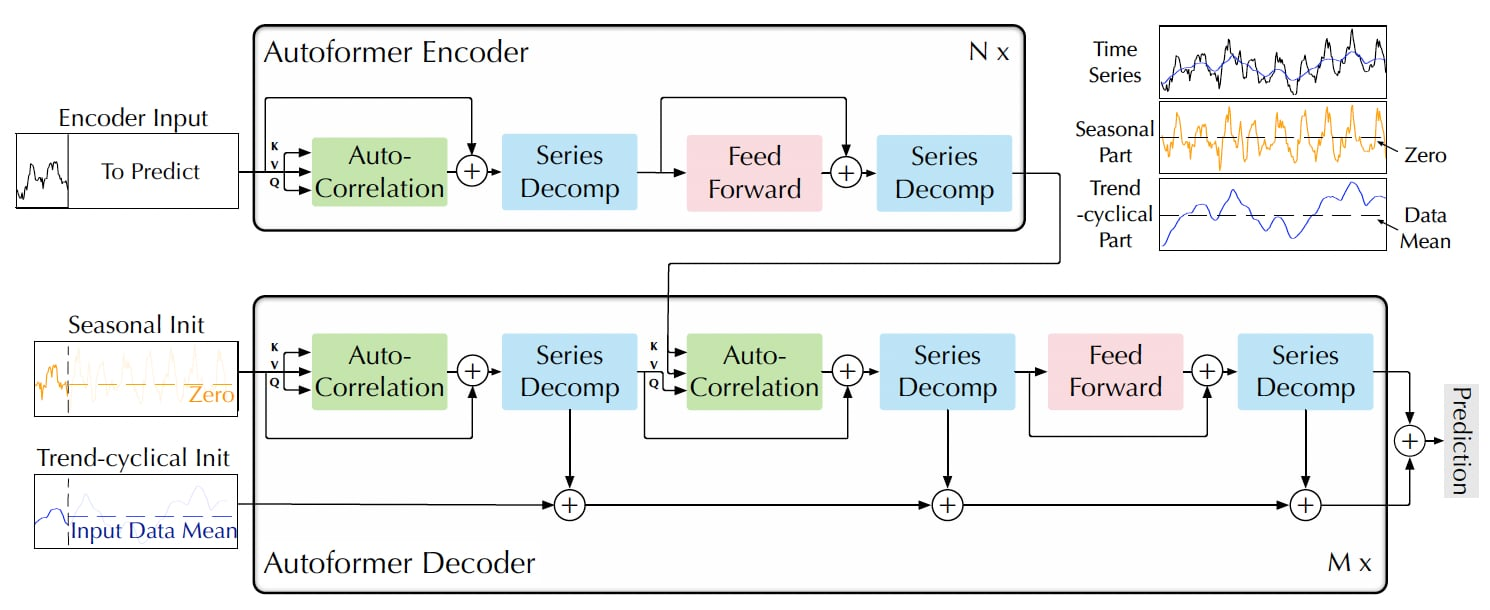
\includegraphics[width=0.4\textwidth]{img/autoformer.jpg}}
\caption{Tổng quan mô hình Autoformer.}
\label{fig}
\end{figure}

Decomposition Layer – lớp phân rã được tạo ra để nhằm nâng cao khả năng mô hình phân tách các thành phân trên chính xác hơn. Autoformer giới thiệu 1 phương pháp tự động tương quan (Autocorrelation) cải tiến để thay thế cho self-attention trong mô hình Transformer chuẩn. Cơ chế tự động tương quan này cho phép mô hình tận dụng sự phụ thuộc theo thời gian, từ đó cải thiện hiệu suất của mô hình tổng thể.

\begin{figure}[htbp]
\centerline{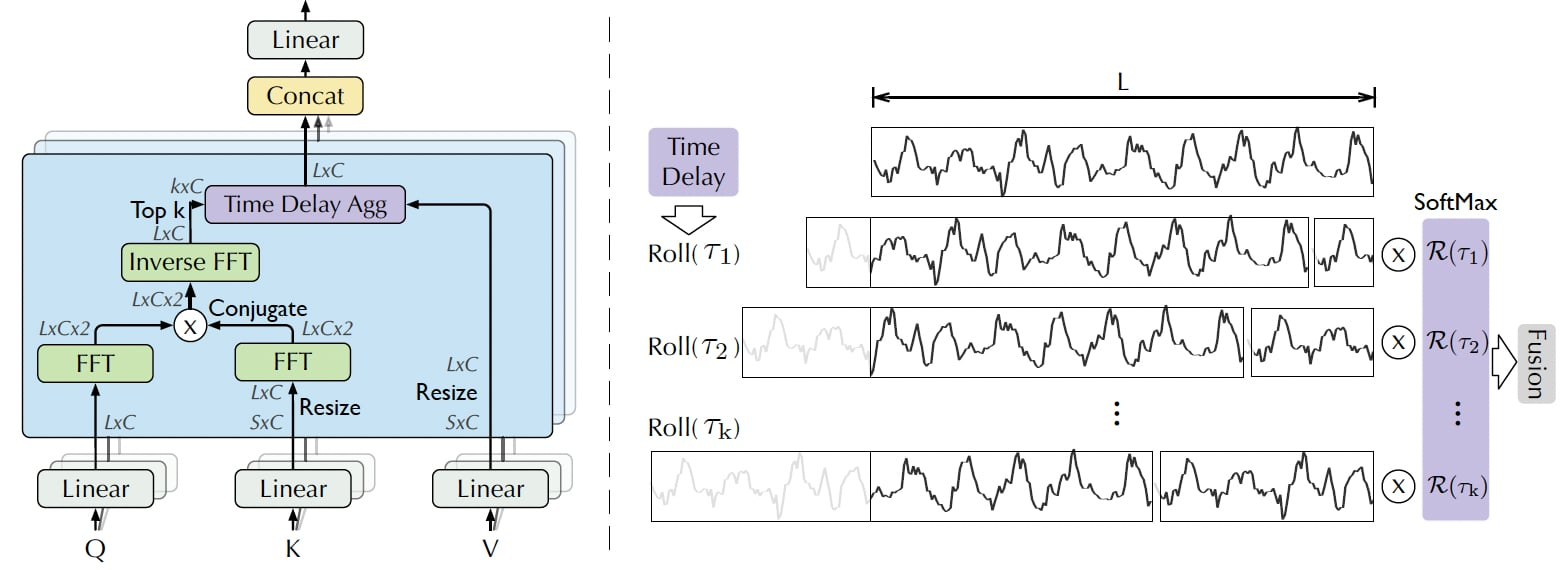
\includegraphics[width=0.4\textwidth]{img/autocorrelation.jpg}}
\caption{Cơ chế autocorrelation.}
\label{fig}
\end{figure}